\documentclass{article}
\usepackage{graphicx}
\usepackage[utf8]{inputenc}
\usepackage{amsmath}
\usepackage{amssymb}
\usepackage{graphicx}
\usepackage{epstopdf}
\usepackage{inputenc}
\usepackage{latexsym}
\usepackage{setspace}
\usepackage{caption}
\usepackage{authblk}
\usepackage{float}
\setlength\parindent{24pt}
\usepackage[export]{adjustbox}


\begin{document}

\title{Muon Decay Measurements Using Commercial Electronics}
\author{Loïc James McKeever}
\affil{Mackenzie Levangie}

\maketitle

\section{Introduction}

In this experiment we attempt to determine the mean lifetime of muons.  This will be done by detecting muons and muon decays using a scintillator detector and specialized software.  The data will be filtered to only the detection of decays. Once filtered the data is binned and curve fit using the Maximum Likelyhood and Least Squares methods.  We will test both methods on a sets of data we simulate ourselves.  We found a mean lifetime of $2.03 \mu s \pm 0.06 \mu s$ which agrees with the expected value of somewhere between $2.043 \mu s$ (for negative muons) and $2.197 \mu s$ (for positive muons).   

\section{Materials and Methods}

This experiment had two main parts.  One part consisted of detecting muons using a scintillator and collecting timing data for each detection to later determine whether or not the muon had decayed.  The second part consisted of simulating a certain number of muon decays using code written ourselves.

Using the set up shown in Figure 1$^{[1]}$ we were able gather timing data for each muon detected by the scintillator using muon software designed for the experiment.  A multimeter(GW Instek GDM-8341X2) was used to monitor the high voltage power(HV) which was kept at -1150 V for the duration of the experiment.  A second multimeter(same make and model) connected to the discriminator was used to monitor the threshold which was set at 200mV.  The optimal threshold was determined by varying its value attempting to approach the expected muon rate of ~7 muons/s (based on the flux at sea level$^{[2]}$, the height of the scintillator$^{[3]}$ and incoming angle of the muons$^{[4]}$.  Below the optimal threshold and we don't detect some decays and above it we get too many false positives.  We also used a 2 channel oscilloscope(Tektronix TDS210) to ensure we were getting a signal from the photo-multiplier tube(PMT) and the discriminator.  

\begin{figure}[H]
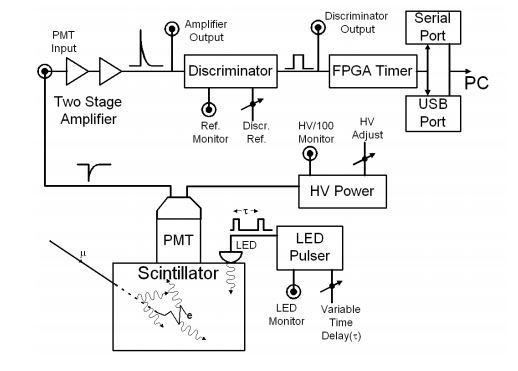
\includegraphics[scale=0.75,center]{MuonSetup.JPG}
\caption{This figure shows the experimental setup used in this lab.}
\end{figure}

Once the equipment was setup it was left to gather data from 3000 separate muon decays.  While the data was being gathered we wrote a program that allowed us to simulate a given number of muon decays.  This was done simply by taking n random samples determined by $t_i=-\tau ln(r_i)^{[5]}$ where $t_i$ is our decay time, $\tau$ is our theoretical muon lifetime(here 2.2 $\mu s$) and $r_i$ is a random number between 0 and 1.  Once that data has been simulated a specific number of times the program will then curve fit the data using the Maximum Likelyhood method(ML) and the Least Squares method(LS).  We simulated both 500 decays and 3000 decays.

After the experimental data was gathered it then needed to be "cleaned" because the data included muons that did not decay(~520 000).  This was done by a program we wrote that reads each data point and only saves it if the decay time is less than 40000 microseconds(timing window of the apparatus).  We also wrote a separate program that used ML and LS methods to curve fit our data to then determine our mean lifetime.  We curve fit both the entirety of our data and disjoint sets of 500 points each.

\section{Results}

We wrote a program in Matlab that given a certain input will simulate that number of muon decays based on the known mean lifetime of $2.2 \mu s$.  We ran this simulation for 500 decays(Figure 2) and then for 3000 decays(Figure 3).  The data was binned into 50 ns bins.  The curve fits were obtained using ML and LS methods and then mean lifetime was determined numerically as where the errors(plus $2\sigma$ for the ML and $\chi^2+1$ for the LS).  

\begin{figure}[H]
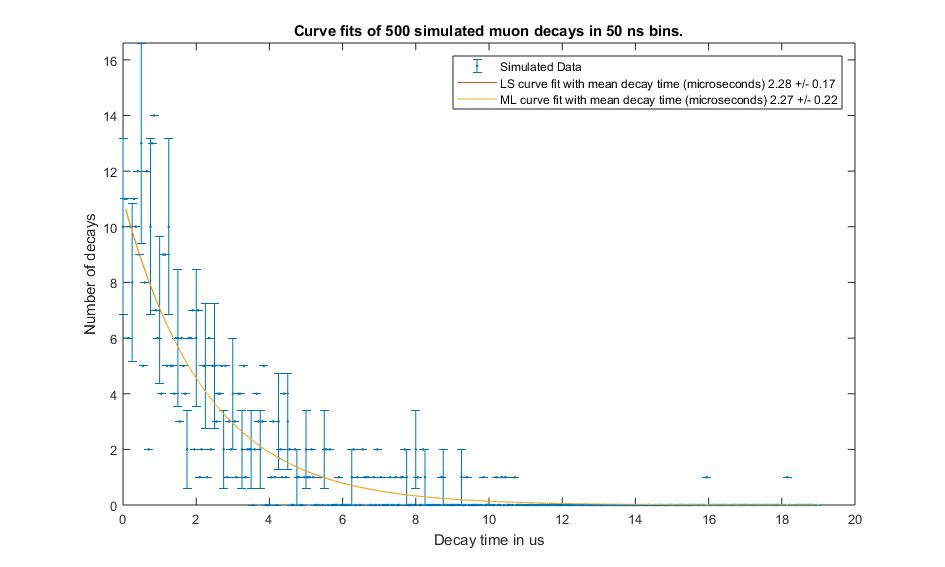
\includegraphics[scale=0.6,center]{Simulated_500.jpg}
\caption{This figure shows the binned data from 500 simulated muon decays.  For visibility every fifth data point has its error bars showing.  Both curve fitting methods gave very similar results; a mean lifetime of $2.28 \pm 0.17 \mu s$ for the LS and $2.27 \pm 0.22 \mu s$.  Both agree with the expected value of $2.2 \mu s$.}
\end{figure}

\begin{figure}[H]
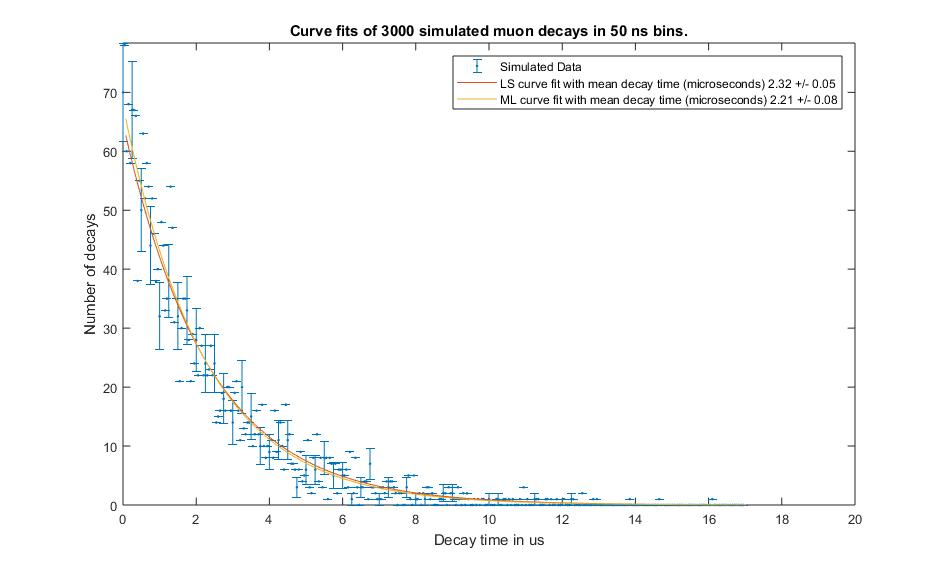
\includegraphics[scale=0.6,center]{Simulated_3000.jpg}
\caption{This figure shows the binned data from 3000 simulated muon decays.  For visibility every fifth data point has its error bars showing.  This time the curve fits give relatively different results; a mean lifetime of $2.32 \pm 0.05 \mu s$ for the LS and $2.21 \pm 0.08 \mu s$.  So the LS method might be more precise than the ML method but it's less accurate and doesn't agree with the expected value.}
\end{figure}

The final program we wrote took the cleaned data and binned, plotted and curve fit it using the same methods as the simulation program(ML and LS)  as well as the same method of calculating the errors.  The 3000 data points were binned and plotted all together and curve fit using the ML method(Figure 4) and the LS method(Figure 5).  The data was then divided into sets of 500 points and those sets were binned, plotted and curve fit using only the ML method(Figures 6 through 11).

\begin{figure}[H]
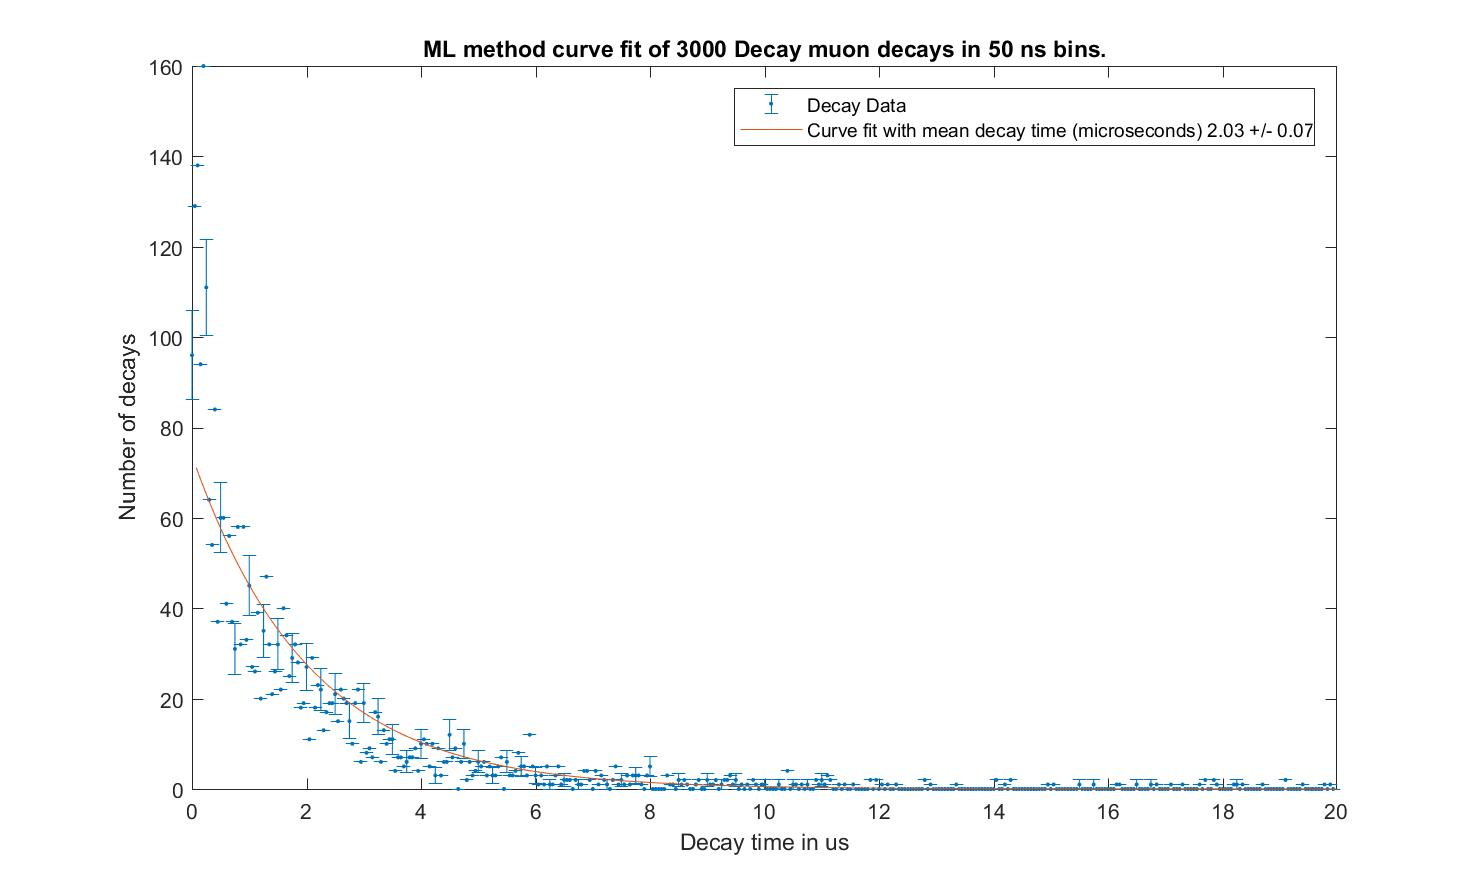
\includegraphics[scale=0.4,center]{ML_Curve_Fit_3000.jpg}
\caption{This figure shows the ML curve fit of our 3000 muon decays.  For visibility every fifth data point has its error bars showing.  The mean lifetime was calculated to be $2.03 \pm 0.07$ which agrees with the expected value of somewhere between $2.043 \mu s$ (for negative muons) and $2.197 \mu s$ (for positive muons).}
\end{figure}

\begin{figure}[H]
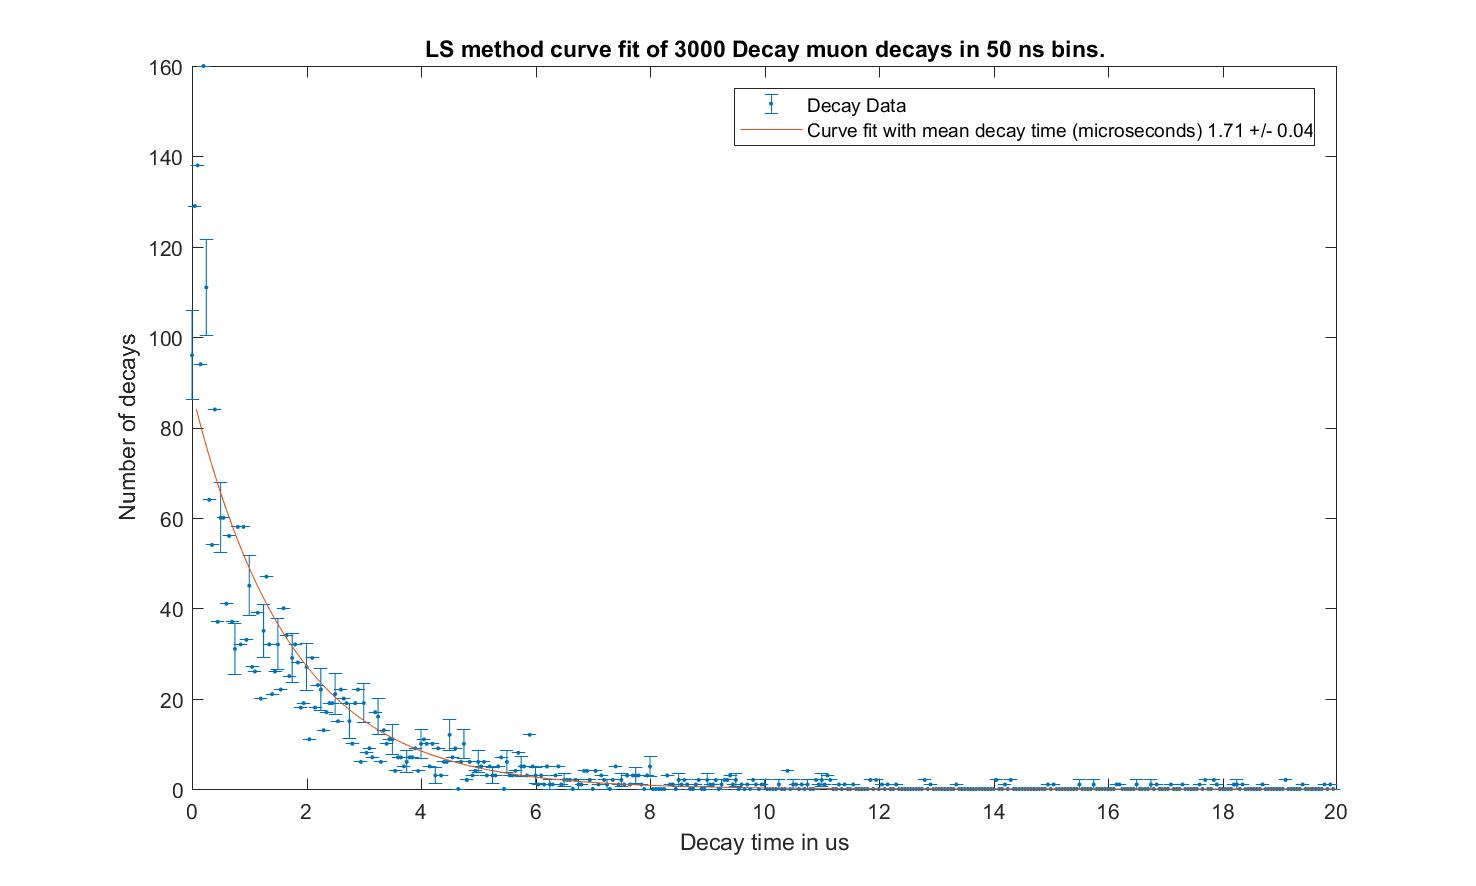
\includegraphics[scale=0.4,center]{LS_Curve_Fit_3000.jpg}
\caption{This figure shows the ML curve fit of our 3000 muon decays.  For visibility every fifth data point has its error bars showing.  The mean lifetime was calculated to be $1.71 \pm 0.04$ which does not agree with the expected value of somewhere between $2.043 \mu s$ (for negative muons) and $2.197 \mu s$ (for positive muons).  Again the LS method seems to be more precise while being less accurate.}
\end{figure}
 
\begin{figure}[H]
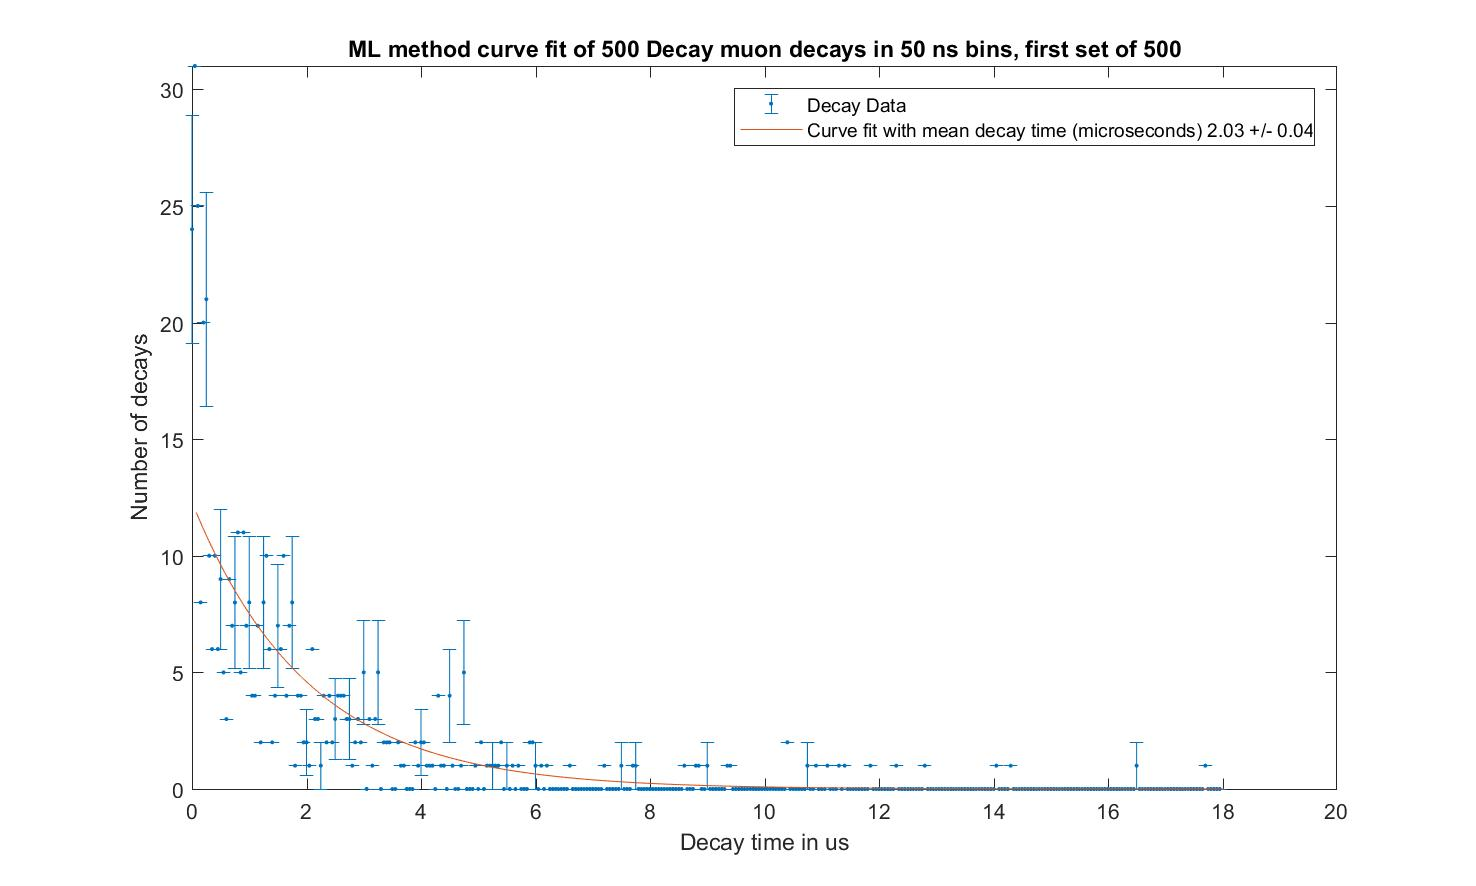
\includegraphics[scale=0.4,center]{ML_Curve_Fit_500a.jpg}
\caption{This figure shows the ML curve fit of our first set of muon decays.  For visibility every fifth data point has its error bars showing.  The mean lifetime was calculated to be $2.03 \pm 0.04$ which agrees with the expected value of somewhere between $2.043 \mu s$ (for negative muons) and $2.197 \mu s$ (for positive muons).}
\end{figure}

\begin{figure}[H]
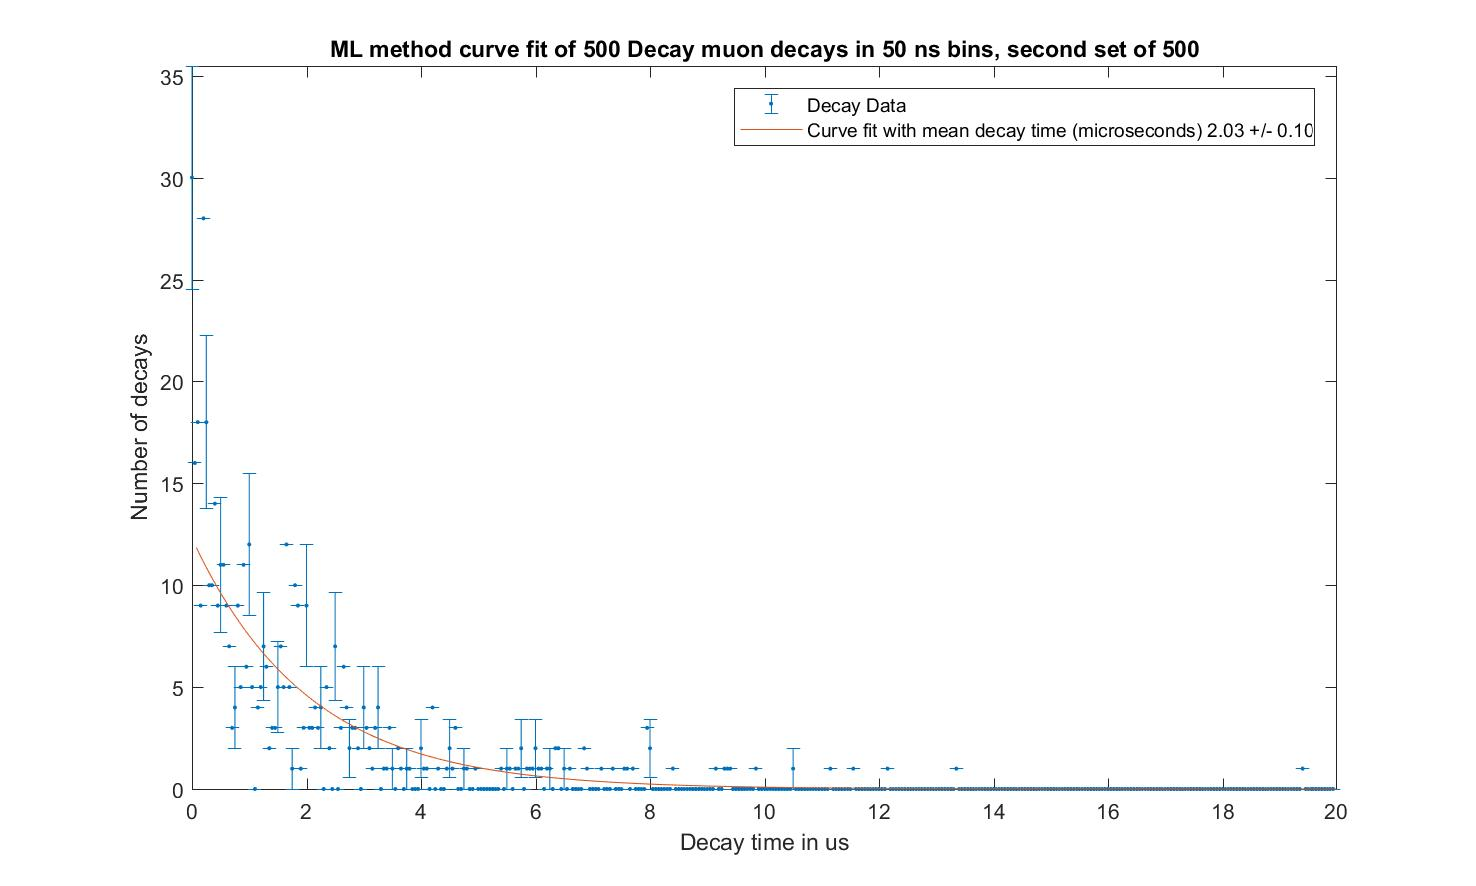
\includegraphics[scale=0.4,center]{ML_Curve_Fit_500b.jpg}
\caption{This figure shows the ML curve fit of our first set of muon decays.  For visibility every fifth data point has its error bars showing.  The mean lifetime was calculated to be $2.03 \pm 0.10$ which agrees with the expected value of somewhere between $2.043 \mu s$ (for negative muons) and $2.197 \mu s$ (for positive muons).}
\end{figure}

\begin{figure}[H]
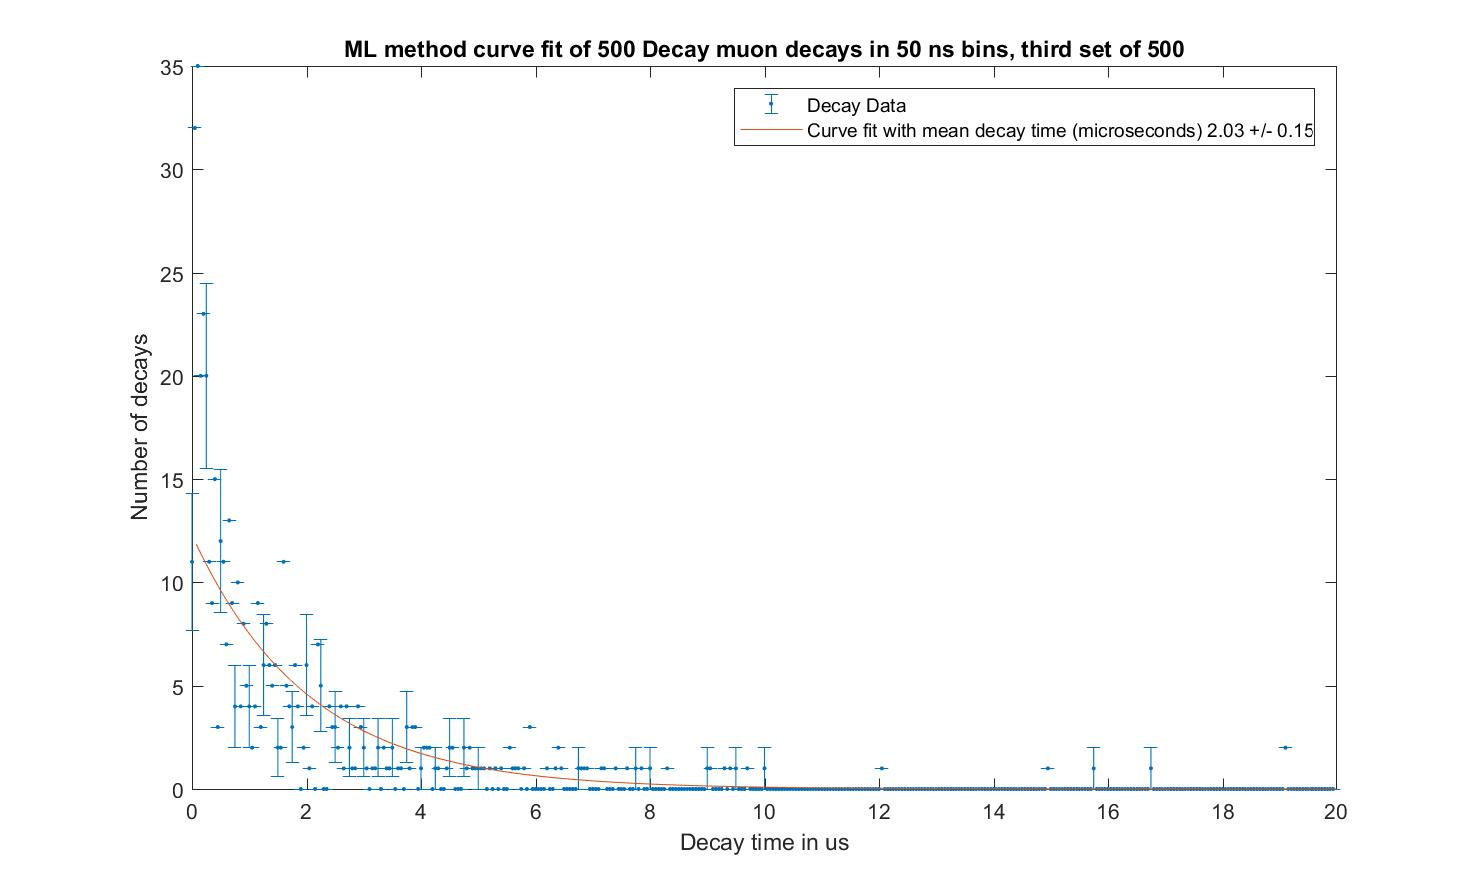
\includegraphics[scale=0.4,center]{ML_Curve_Fit_500c.jpg}
\caption{This figure shows the ML curve fit of our first set of muon decays.  For visibility every fifth data point has its error bars showing.  The mean lifetime was calculated to be $2.03 \pm 0.15$ which agrees with the expected value of somewhere between $2.043 \mu s$ (for negative muons) and $2.197 \mu s$ (for positive muons).}
\end{figure}

\begin{figure}[H]
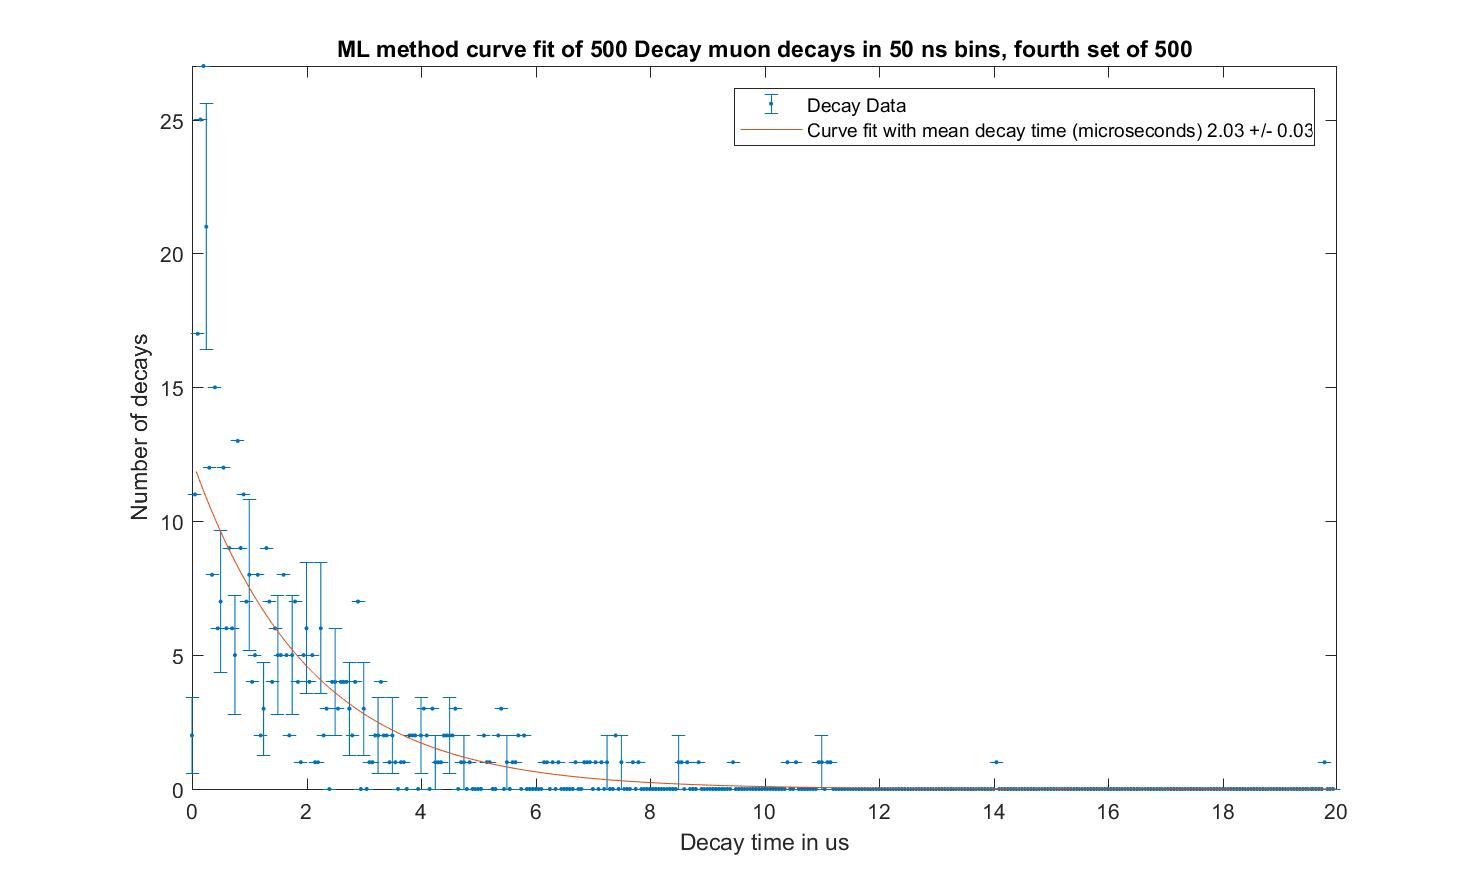
\includegraphics[scale=0.4,center]{ML_Curve_Fit_500d.jpg}
\caption{This figure shows the ML curve fit of our first set of muon decays.  For visibility every fifth data point has its error bars showing.  The mean lifetime was calculated to be $2.03 \pm 0.03$ which agrees with the expected value of somewhere between $2.043 \mu s$ (for negative muons) and $2.197 \mu s$ (for positive muons).}
\end{figure}

\begin{figure}[H]
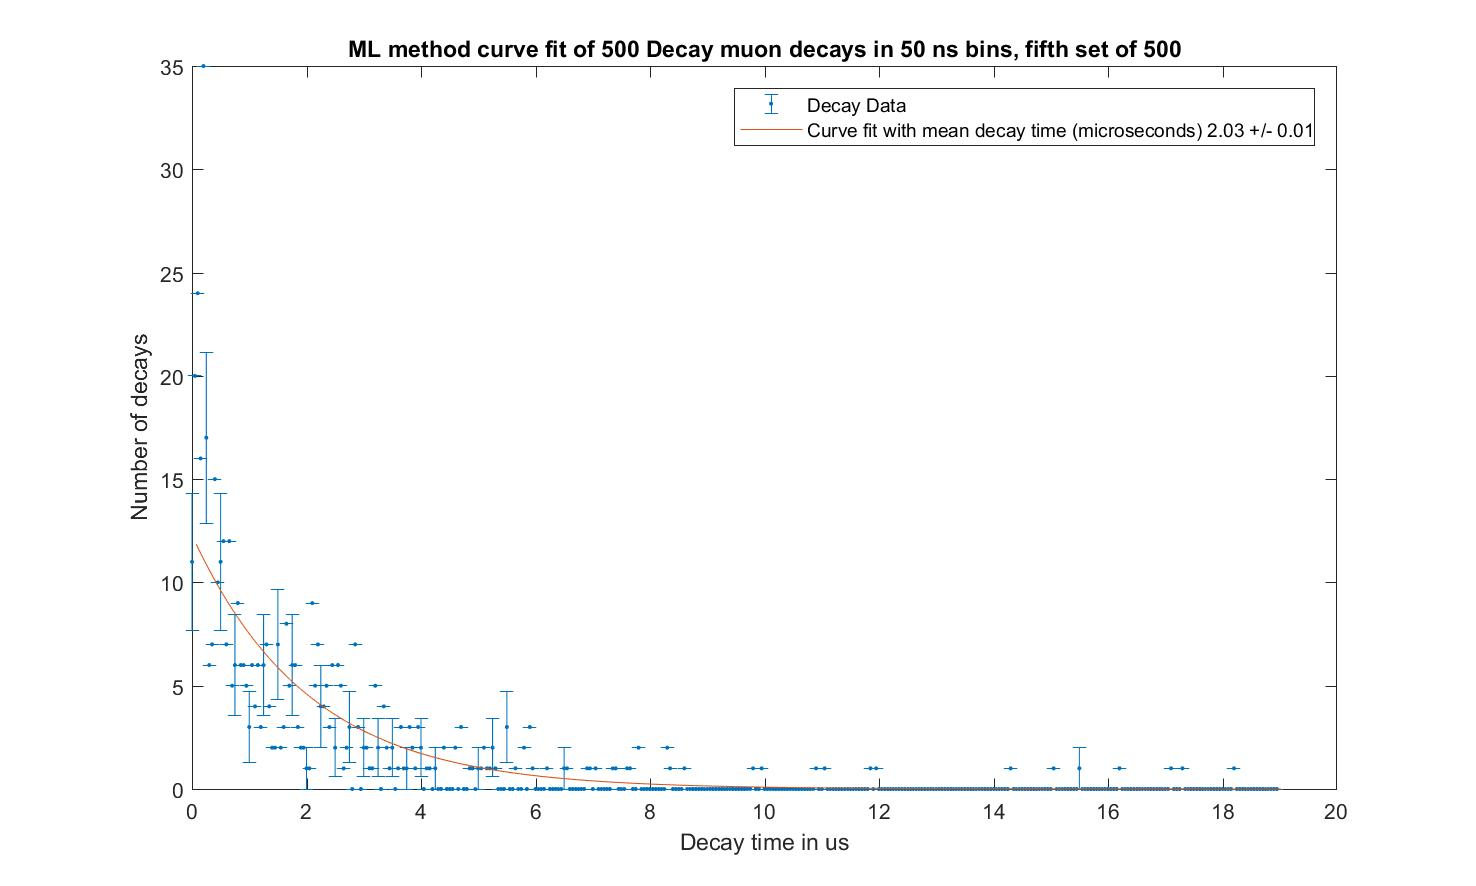
\includegraphics[scale=0.4,center]{ML_Curve_Fit_500e.jpg}
\caption{This figure shows the ML curve fit of our first set of muon decays.  For visibility every fifth data point has its error bars showing.  The mean lifetime was calculated to be $2.03 \pm 0.01$ which agrees with the expected value of somewhere between $2.043 \mu s$ (for negative muons) and $2.197 \mu s$ (for positive muons).}
\end{figure}

\begin{figure}[H]
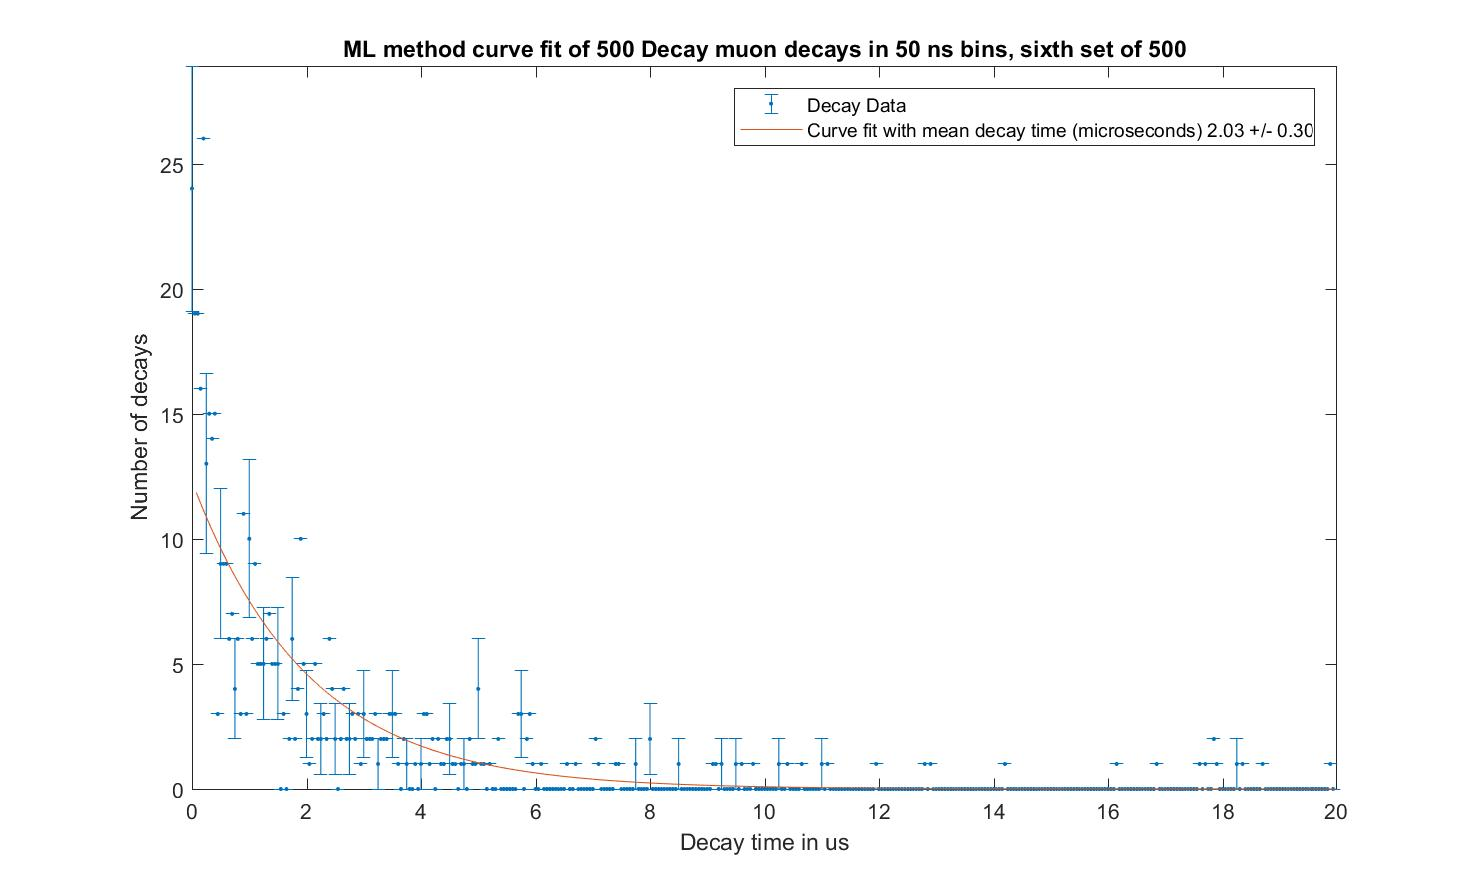
\includegraphics[scale=0.4,center]{ML_Curve_Fit_500f.jpg}
\caption{This figure shows the ML curve fit of our first set of muon decays.  For visibility every fifth data point has its error bars showing.  The mean lifetime was calculated to be $2.03 \pm 0.30$ which agrees with the expected value of somewhere between $2.043 \mu s$ (for negative muons) and $2.197 \mu s$ (for positive muons).}
\end{figure}

\section{Discussion}

Based on the simulation data and the experimental data the ML method seems to be better suited than the LS method for this type of experiment(perhaps it has something to do with the need to linearize the data) and is much more accurate despite being slightly less precise.  The ML method agreed with expected results for both simulations performed while the LS only agreed with our expected value for our first simulation of 500 decays.  We can calculate the mean lifetime based on the six results obtained when we divided our experimental data up and we find $\tau=2.03 \mu s \pm 0.06$ which agrees with the expected value of somewhere between $2.043 \mu s$ (for negative muons) and $2.197 \mu s$ (for positive muons) within our uncertainty.  Given a certain ratio of positive to negative muons we could determine the exact value we'd would expect.  Should the experiment be repeated a more accurate determination of the threshold voltage on the discriminator would undoubtedly improve results.  

\section{Conclusions}

In conclusion we were able to accurately determine the mean life time of two sets of simulated data using the Maximum Likelyhood method.  We expected a value of $2.2 \mu s$ and found $2.27 \pm 0.22 \mu s$ and $2.21 \pm 0.08 \mu s$ for simulations of 500 and 3000 decays respectively.  We were then able to use this curve fitting method to determine the mean lifetime of a set of experimental data.  We gathered 3000 data points and found a mean lifetime of $2.03 \pm 0.07 \mu s$ and did the same after dividing our data into sets of 500 and found $\tau=2.03 \pm 0.06 \mu s$ both of which agree with the expected value of somewhere between $2.043 \mu s$ and $2.197 \mu s$.

\section{References}


[1] Figure 5, Muon Physics Lab Manual, T.E. Coan and J. Ye 

\noindent[2] Introduction, Muon Physics Lab Manual, T.E. Coan and J. Ye

\noindent [3] Specifications, TeachSpin Muon Physics https://www.teachspin.com/muon-physics

\noindent[4] Measuring the Angular Distribution of Muons, Inna Shteinbuk

\noindent[5] Chapter 5 Section 3,  Data Reduction and Error Analysis, P. R. Bevington and D. Robinson

\section{Appendix}

See code attached below.

\end{document}
